\documentclass [a4paper, 12pt]{article}
\usepackage {amssymb, amsmath}
\usepackage {graphicx}
\usepackage {subcaption}
\usepackage {wrapfig}
\usepackage {float} 
\usepackage {here}
\newtheorem {theorem} {Theorem}
\newtheorem {lemma} {Lemma}
\newtheorem {proposition} {Proposition}
\newtheorem {corollary} {Corollary}
\newtheorem {definition} {Definition}
\newtheorem {notation} {Notation}

\begin {document}
\title{Multigrid Algorithm}

\author{Quincy Gu \thanks {Research guided by 
Prof. jeffery Calder's guidance for MATH 4997W, Senior Project for undergraduate mathematics major students at the 
University of Minnesota.} \\
Department of Mathematics \\
University of Minnesota-Twin Cities \\
Minneapolis, Minnesota 55455 \\
\texttt {guxxx504@umn.edu}}

\date{\today}

\maketitle

\begin {abstract}

In this paper, I focused on the general concepts of the multigrid algorithm, and compare the Gauss-Seidel, Jacobi and Multigrid Algorithms with different data. In the following part of this paper, I introduced the basic ideas of the multigrid methods, and some specific sample functions involved in the multigrid algorithms.

\end {abstract}

\section {Introduction} \label {S:intro}

Multigrid Methods are mainly used in solving the linear or non-linear partial differential equations, my work here is mainly focused on the iterations of the convergence based on the multigrid algorithm. Since the Gauss-Seidel and Jacobi iterations requires a quite large number of iterations, and we denoted the number of iterations as $n$ here, and in many cases, this $n$ could be a large enough number. In a realistic system, if we try to solve it in a high accuracy with the Gauss-Seidel and Jacobi iterations, it technically takes quite a long time. However, if we solve the system with multigrid methods, it is easier to get more precisely with finite number of iterations, and usually it could get the expected solution with less time. \\
Since our goal is to compare the three above different Partial Differential Equations' solvers (Gauss-Seidel, Jacobi \& Multigrid Algorithms), I prefer to introduce more about the backgrounds of these algorithms. And the following three subsections related to all these algorithms would leave more details about their applications in solving the partial differential equations. Because we only expect to aompare the Multigrid algorithm with the Gauss-Seidel and Jacobi algorithms, I just have two subsections in the following, and combine the Gauss-Seidel and Jacobi algorithms together in one subsection.

\subsection {Gauss-Seidel \& Jacobi Algorithms}
As Randall J. LeVeque mentioned in his work \emph {Finite Difference Methods for Ordinary and Partial Differential Equations: Steady-State and Time-Dependent Problems}, Jacobi and Gauss-Seidel as two classical iterative methods are poor methods in general which converge very slowly when used as standalone methods. He also concluded some important features of these two classical methods, and the last feature he discussed there \footnote {LeVeque, R. (2007). Finite difference methods for ordinary and partial differential equations : Steady-state and time-dependent problems. Philadelphia, Pa.: Society for Industrial and Applied Mathematics}, which indicates that since each iteration based on these two iterative methods require $O(m^2)$ work, then each of these two iterative methods would expect $O(m^2\log m)$ iterations to reach a level of accuracy cpmsistent with the expected global error in the solution. And he pointed out that based on these, if we use either one of these two classical iterative methods, the work per iteration would give a total opertaion count of $O(m^4\log m)$, which would take a lot of the iteration steps and require quite a long time. \\
Base on the discussions above, it is clear enough that why the Jacobi and Gauss-Seidel methods are not good enough in solving the partial differential equations, and these two iterative methods absolutely are not what we preferred to use. But, these two classicial methods could be used to improve the Multigrid Algorithm, which will be introduced in the following subsection. One example in Randall J. LeVeque's book,``the Jacobi Method just could be used as a smoother for the multigrid method" (Randall J. LeVeque, 69) just indicated this. So, even we preferred not using these two classical iterative methods, they still be useful in solving the poisson equations, improving other methods and etc.

\subsection {Multigrid Algorithm}
The Multigrid Method as we introduced in the very beginning of this article, it is much more powerful than the other two classical iterative methods discussed in the previous subsection. Randall J. LeVeque also indicated that the key idea in multigrid is to switch now to a coarser grid to estimate the remaining error. He also pointed out two advantages of the multigrid method in his work, one is itrating on a coarser grid could take less work than iterating further on the original grid, the other is the convergence rate for some components of the error is greatly improved by transferring the error to a coarser grid. And we could get a better understanding about this when we start to discuss the general multigrid algorithm in the following ``Methods" section. \\
Morever, as Achi Brandt and Oren E. Livne mentioned in the book \emph {Multigrid Techniques:\
1984 Guide with Applications to Fluid Dynamics. Revised Edition}, except being the fast partial differential equations' solver, the multigrid method could also be used related to stiffness. It can provide very efficient grid-adaptation procedures for either boundary-value \footnote {The boundary value problem is what we focused on in this article} or evolution problems in which different scales of discretization are needed in different parts of the domain. They pointed out that the multigrid method could not only give new dimension of efficiency to stiff evolution problem, but also could resolve the conflict between higher accuracy and stability in case of non-eliptic and singular perturbation boundary-value problem. In addition to these, they also noticed that the multigrid method could enormously reduce the amount of discrete relations employed in solving chains of similar boundary-value, optimization problems, and integral equations, also, it could be used to vastly cut the required computer storage, since sometimes by several orders of magnitude, the computer resources needed to solve some large systems which do not originate from partial differential or integral equations. \footnote {Brandt, A., \& Livne, O. (2011): Multigrid Techniques: \
1984 guide with applications to fluid dynamics. Rev. ed. Philadelphia: Society for Industrial and 
Applied Mathematics} \\
Base on all these above, we could get an intution that the multigrid algorithm is the iterative method that is powerful applied in solving any partial differential equations related problems.

\section {Methods}

\subsection {General Overview}

First, we set a simple two-dimensional model of the poisson equation as the initial case to adapt the multigrid algorithm. Let \\
\begin {equation}
       Poisson \ Equation=
       \begin {cases}
             -\Delta u=f,      &\text {if in $(0,1)^2$;} \\
             u=0,                 &\text {if on $\partial (0,1)^2$.} 
       \end {cases}
\end {equation}
where \\
\begin {equation}
      \Delta u=\frac {\partial^2 u}
                              {\partial x^2}
                      +
                      \frac {\partial^2 u}
                               {\partial y^2}
                      =U_{xx}+U_{yy}
\end {equation}
Notice that in this case, $u=0$ means the following: \\
\begin {equation}
      \Longrightarrow 
      \begin {cases}
            u(x,1)=0; \\
            u(x,0)=0; \\
            u(1,y)=0; \\
            u(0,y)=0.
      \end {cases}
\end {equation}
Based on these, we could solve for finite different schemes, then we could have the following \\
\begin {equation}
      f'(x)=\lim_{h \to 0} \frac {f(x+h)-f(x)}
                                              {h}
\end {equation}
Then, we set up two subcases, based on the value of h is positive or negative. Let the case when $h>0$ be ``Forward Difference". On the contrary, let the case with 
$h<0$ be ``Backward Difference". \\
$(i). h>0:$ \\
\begin {equation}
      f'(x) \equiv \frac {f(x+h)-f(x)}
                                  {h}
\end {equation} \\
$(ii). h<0:$ \\
\begin {equation}
      f'(x) \equiv \frac {f(x)-f(x-h)}
                                  {h}
\end {equation}
Based on these, we could calculate the grid for both the two cases, which are \\
\begin {equation}
      f'_i \simeq \frac {f_{i+1}-f_i}
                                 {h}
\end {equation}
or \\
\begin {equation}
      f'_i \simeq \frac {f_i-f_{i-1}}
                                 {h}
\end {equation}
From all the above, we could generate the second derivatives of $f_i$ of the problem \\
\begin {equation}
      \Longrightarrow
      \begin {cases}
s[u]_{ij}=0, &\text{$1<i<n, 1<j<n$;} \\
u_{ij}=0; \\
u_{nj}=0; \\
u_{i1}=0; \\
u_{in}=0.
      \end {cases}
\end {equation}
which is the following: \\
\begin {alignat}{3} \label {E:mm4}
f''_i &= \frac {f'_{i+1}-f'_i}
                     {h} \\
       &=\frac {(\frac{f_{i+1}-f_i}
                     {h})-(\frac{f_i-f_{i-1}}
                                      {h})}
                     {h} \\
       &=\frac {f_{i+1}-2f_i+f_{i-1}}
                     {h^2}
\end {alignat}
Finally, we could get \\
\begin {equation}
      f''(x)=\frac {f(x+h)-2f(x)+f(x-h)}
                         {h^2}
              +
                0(h^2)
\end {equation}
as the general solution for our initial case differential poisson equation.
From our initial case, then get a more complex $2-dimensional$ model, using the similar methods, we could generate the final solution as \\
\begin {equation}
S[u]_{ij}= \frac {u_{i+1,j}-2u_{ij}+u_{i-1,j}}
                         {h^2}
                +
                \frac {u_{i,j+1}-2u_{ij}+u_{i,j-1}}
                         {h^2}
                +f_{ij}
\end {equation}
After these above two simple test cases and the previous subsection contents, we could generate the general processes about the Multigrid Algorithm (Or, Multigrid Methods). As Dr. Randall J. LeVeque's depictions in his book \emph {Finite Difference Methods for Ordinary and Partial Differential Equations: Steady-State and Time-Dependent Problems}, he pointed out six steps for the multigrid approach. I listed in the following \footnote {LeVeque, R. (2007). Finite difference methods for ordinary and partial differential equations : Steady-state and time-dependent problems. Philadelphia, Pa.: Society for Industrial and Applied Mathematics}: 
\begin {enumerate}
\item Take a fixed number of iterations ($e.g., v=3$) of a simple iterative method ($e.g.$, underrelaxed Jacobi or another choice of ``smoother") on the original 
$m \times m$ system $Au=f$. This gives an approximation $U_v \in \Re^m$. \\
\item Compute the residual $r_v=f-Au_v \in \Re^m$. \\
\item Coarsen the residual: approximate the grid function $r_v$ on a grid with $m_c=(m-1)/2$ points to obtain $\tilde{r} \in \Re^{m_c}$. \\
\item Approximately solve the system $\tilde{A} \tilde{e}=-\tilde{r}$, where $\tilde{A}$ is the $m_c \times m_c$ version of $A$ (the tridiagonal approximation to 
$d^2 / dx^2$ on a grid with $m_c$ points). \\
\item The vector $\tilde{e}$ approximates the error in $u_v$ but only at $m_c$ points on the coarse grid. Interpolate this grid function back to the original grid with 
$m$ points to obtain an approximation to $e_v$. Subtract this form $u_v$ to get a better approximation to $u^*$. \\
\item Using this as a starting guess, take a few more iterations ($e.g., v=3$) of a simple iterative method ($e.g.$, underrelaxed Jacobi) on the original $m \times m$ system $Au=f$ to smooth out errors introduced by this intepolation procedure. 
\end {enumerate}
All these above are the general overview about the multigrid algorithm, which contains the initial case of the poisson differential equations, and the general approaches of the multigrid methods. However, since I mentioned the forward and backward differences in the first subsection, I have to clarify this with more details about the finite difference approximations in the following subsection.

\subsection {Finite Difference Approximation}
Based on the general approaches about the multigrid methods in Dr. Randell J. LaVeque's book, also with the forward and backward differences mentioned in the previous subsection, I set the initial case function as the following \\
\begin {equation}
      \begin {cases}
           Au=f. \\
           r=f-Au. \\
      \end {cases}
\end {equation}
to discuss the finite difference approximation with more details in this subsection. \\
Before we start to focus on the finite approximation, the quick review about the gradient descent here is quite beneficial to better understand the poisson iterative methods. \\
For a simple initial case of the poisson equation as \\
\begin {equation}
      \begin {cases}
            U^0_{ij}=0,  &\text {$Considering \ it \ as \ the \ starting \ point$;} \\
            U^{n+1}_{ij}=U^n_{ij}+\Delta tS[U^n]_{ij}; \\
            U^{n+1}_{ij}=0,  &\text {$Considering \ this \ on \ the \ boundary$.} \\
      \end {cases}
\end {equation}
Based on these, keep running with the iterative methods until $U^{n+1}_{ij}=U^n_{ij}$, then we have $S[U^n]_{ij}=0$, which indicate that \\
\begin {equation}
      |S[U^n]_{ij}| \leqslant \varepsilon 
\end {equation}
where $\varepsilon=h^2$.
Now, we continue discussing the finite approximation. To generate the basic multigrid algorithm, we choose $\Delta x$ and some other iterative methods listed in the following \\
\begin {equation}
\begin {cases}
     -Jacobi \& \ Gauss-Seidel; \\
     -Gradient Descent \Longleftrightarrow U_{k+1}=u^k-\Delta t(f-Au). \\
\end {cases}
\end {equation}
as our initial case, which is called $1-vcycle$, and denoted as $U^k$, where the general iterative methods to find its finite approximation has the following four iterable steps: 
\begin {enumerate}
\item Iterating those methods mentioned above for $T_1$ times at $\Delta x (Au=f)$, compute $r^k=f-Au^k$; \\
\item Subsample to $\frac {\Delta x}
                                                                   {2}$,
denoted as $v_k$, iterate the methods for $T_2$ times at $\frac {\Delta x}
                                                                                                              {2}$
to solve $Av^k=r^k$; \\
\item Interpolate $v^k$ back to $\Delta x$ mesh and set \\
\begin {equation}
     u^{k+1}=u^k+v^k
\end {equation} \\
\item Back to the first step. 
\end {enumerate}
Similarly, we could get our initial case be more complexed, where we could have $2-vcycle$ till $n-vcycle$, where $n$ could be any positive integers based on the user's preferences. And we just list the $6$ general steps for the $2-vcycle$ as the example in the following:
\begin {enumerate}
\item Iterating those methods mentioned above for $T_1$ times at $\Delta x (Au=f)$, compute $r^k=f-Au^k$; \\
\item Subsample to $\frac {\Delta x}
                                                                   {2}$,
denoted as $v_k$, iterate the methods for $T_2$ times at $\frac {\Delta x}
                                                                                                              {2}$
to solve $Av^k=r^k$; \\
\item Compute the residual, which is \\
\begin {equation}
      s^k=r^k-Av^k
\end {equation}
Subsample $s^k$ to $\frac {\Delta x}
                                              {4}$,
denoted as $w$, and solve \\
\begin {equation}
      Aw=s^k
\end {equation}
with $T_3$ iterations at those above methods; \\
\item Interpolate $w$ back to $\frac {\Delta x}
                                                                               {2}$
mesh and set \\
\begin {equation}
      v^{k+1}=v^k+w
\end {equation}
\item Iterate $T_2$ times at $\frac {\Delta x}
                                                                             {2}$
mesh starting from $v^{k+1}$, generates $v^{k+1}$; \\
\item Interpolate $v^{k+1}$ to $\Delta x$ mesh, add to $u^k$, which is similar to the third step. 
\end {enumerate}
From all these discussed above, we could get the basic idea of the multigrid algorithm, and how it could be used in the linear or non-linear PDE approximations. We would discuss it with some examples in the folllowing sections of this paper.

\section {Results}
In this section, we write the MatLab code to apply the multigrid algorithm in solving the real world linear or non-linear PDE, and we could get the intutive impression about how the multigrid algorithm take the advantages in the imaging processing related to the partial differential equations. \\
We seperate this section as two subsections, which is related to our previous discussions in the methods section. We first applied the multigrid algorithm with a one-dimensional poisson equation, which is considered as our initial test case, then we publicize this method and applied it in the finite difference approximation, which is considered as the non-linearly differential equations with vcycle and $n$-vcycles.\\
\subsection {Initial Case}
We first testing the Gauss-Seidel and Jacobi algorithms in our initial case, which is the case we discussed in our first part of the ``Methods" section. We set up the function $u$ as the poisson equation we try to solve, which depends on the user input function $f$ and the $\epsilon$. Then we could compute the partial derivatives for $U_{xx}$ and $U_{yy}$, and assign $\Delta u$ equals to $u_{xx}+u_{yy}$. And all the boundary conditions in this case are all the same as we discussed in the first part of the ``Methods" section. Based on these, we write the MatLab code and plot the surface with $X, Y, \& u$, and set our initial iteration count be $0$ and let in increased by $1$ for each iteration. All of these above is our code structure and how we get our surface image optimized. \\
To see how the Jacobi Method applied in solving the partial differential equations with our initial case, we get our input function $f$ be a $100 \times 100$ matrix with all interger $1$, and set the $\epsilon$ value be 0.01. Then it is easy to see that our initial surface is irreguar and have bunch of the huge fluctuations on the ``applicate axis" in this $3D$ graph. To get a first impression about the surface graph at the starting point, I insert it in the following. \\
Then, we run the code, it is obviously that with the finite steps of the iterations, the fluctuations in the ``applicate axis" of the $3D$ surface area would suddenly get smooth, we could compare the following surface plot with the iteration count be $226$ with our surface area at the starting point, and we could find that there are no obvious fluctuations in the $2nd$ plot compared to the $1st$ one. And the surface plot at the $226^{th}$ iteration step is listed together with our first plot. \\
If we continue the iterations, the whole surface area would get to be much more smmother in all of the ``abscissa, ordinate, \& applicate axises". However, if we get a carefully observations for the following surface plots related to each iteration step, there would not have drmatical change between the finite iterations, I also list two surface polts with the iteraton step be $719$ and $1608$ together with the above two surfce plots to get a more clearly impression about how Gauss-Seidel and Jacobi algorithms works in solving a partial differential equation. 
\begin {figure} [h!]
\centering
\begin {subfigure} [b] {0.3\linewidth}
      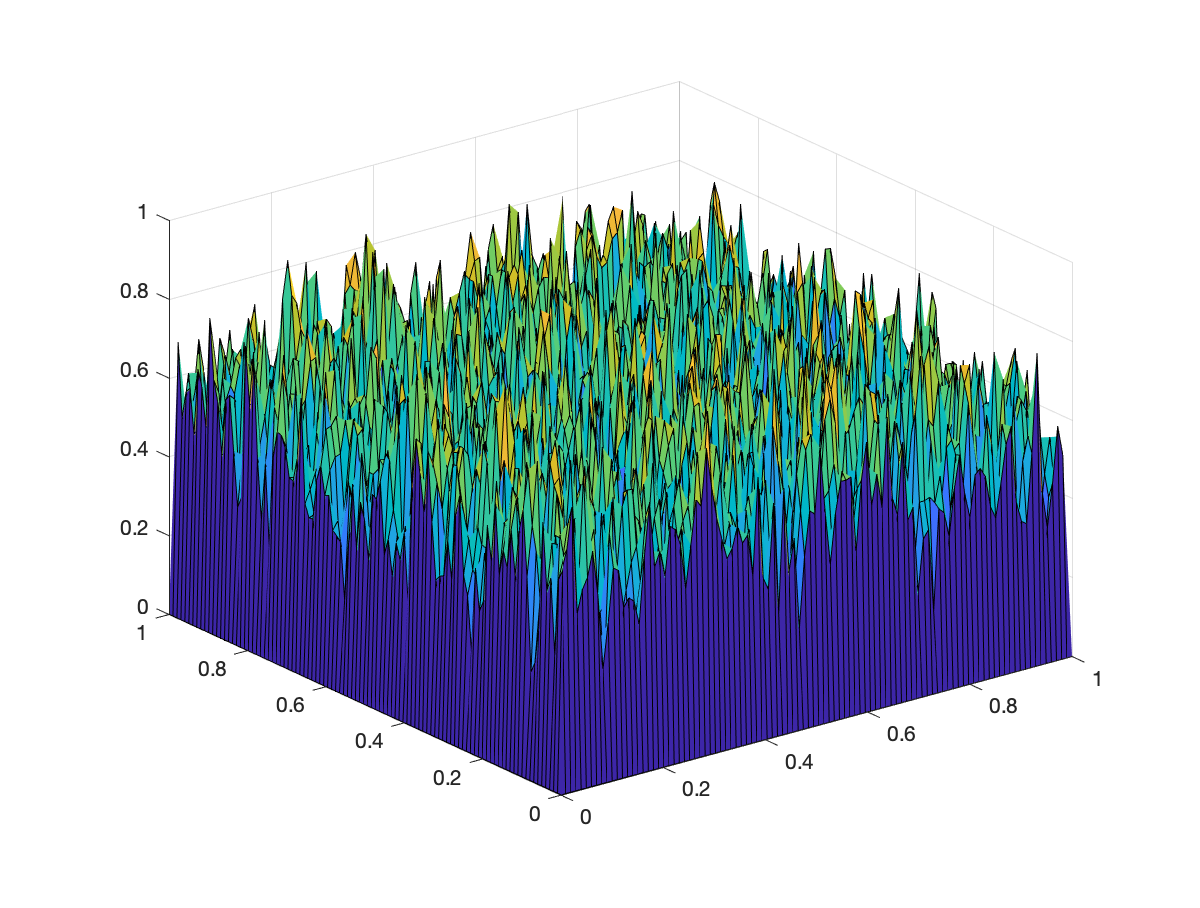
\includegraphics [width=\linewidth] {initial.eps}
      \caption {The Surface Plot at the Starting Point.}
\end {subfigure}
\begin {subfigure} [b] {0.3\linewidth}
      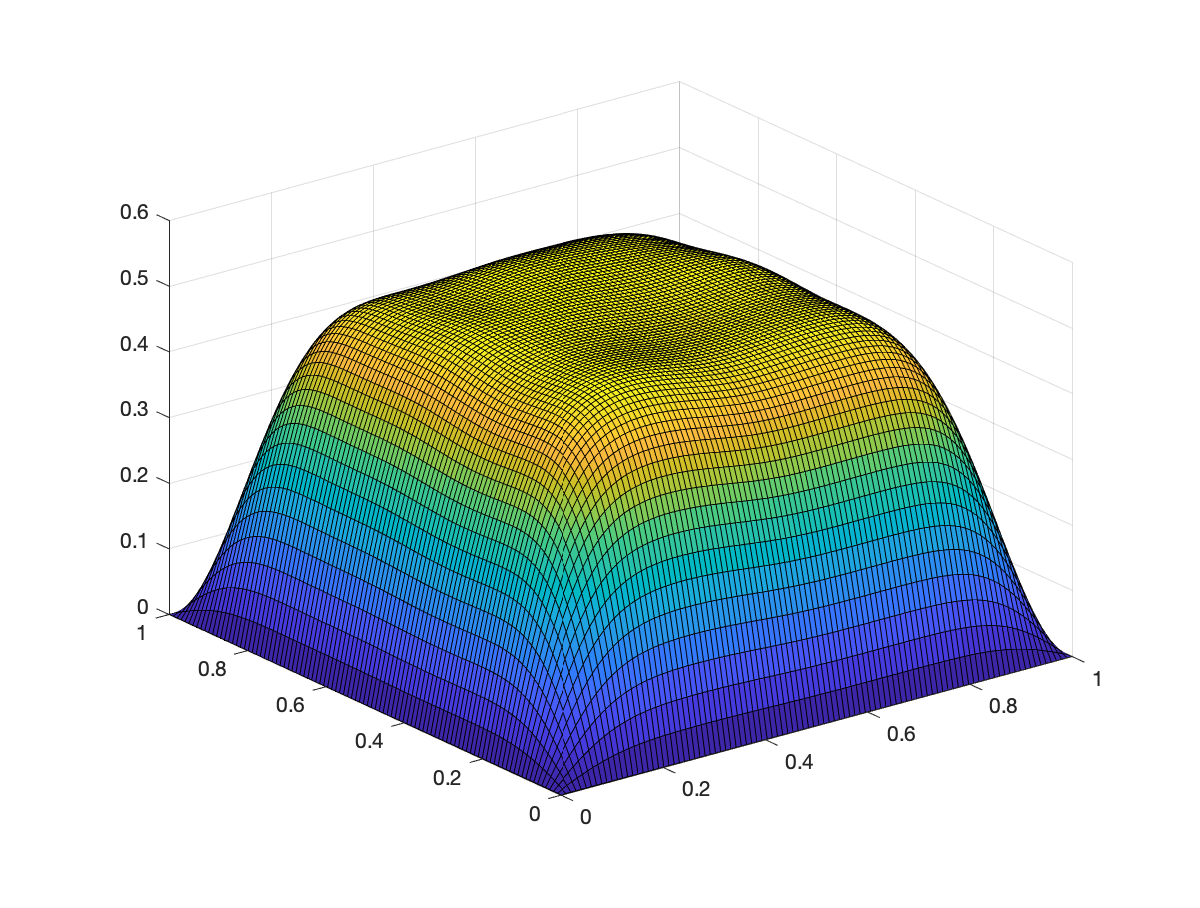
\includegraphics [width=\linewidth] {226.eps}
      \caption {The Surface Plot at the $226^{th}$ Iteration Step.}
\end {subfigure}
\begin {subfigure} [b] {0.3\linewidth}
      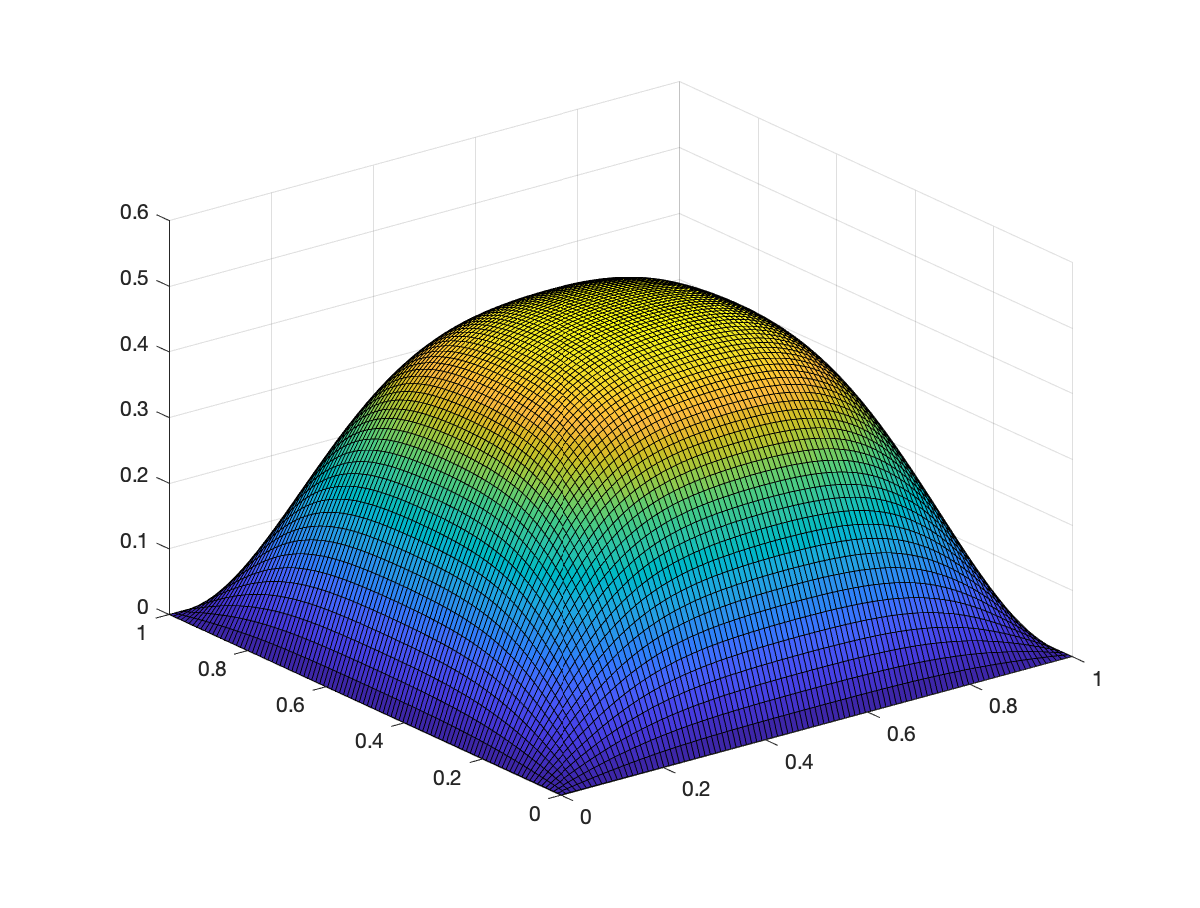
\includegraphics [width=\linewidth] {719.eps}
      \caption {The Surface Plot at the $719^{th}$ Iteration Step.}
\end {subfigure}
\begin {subfigure} [b] {0.3\linewidth}
      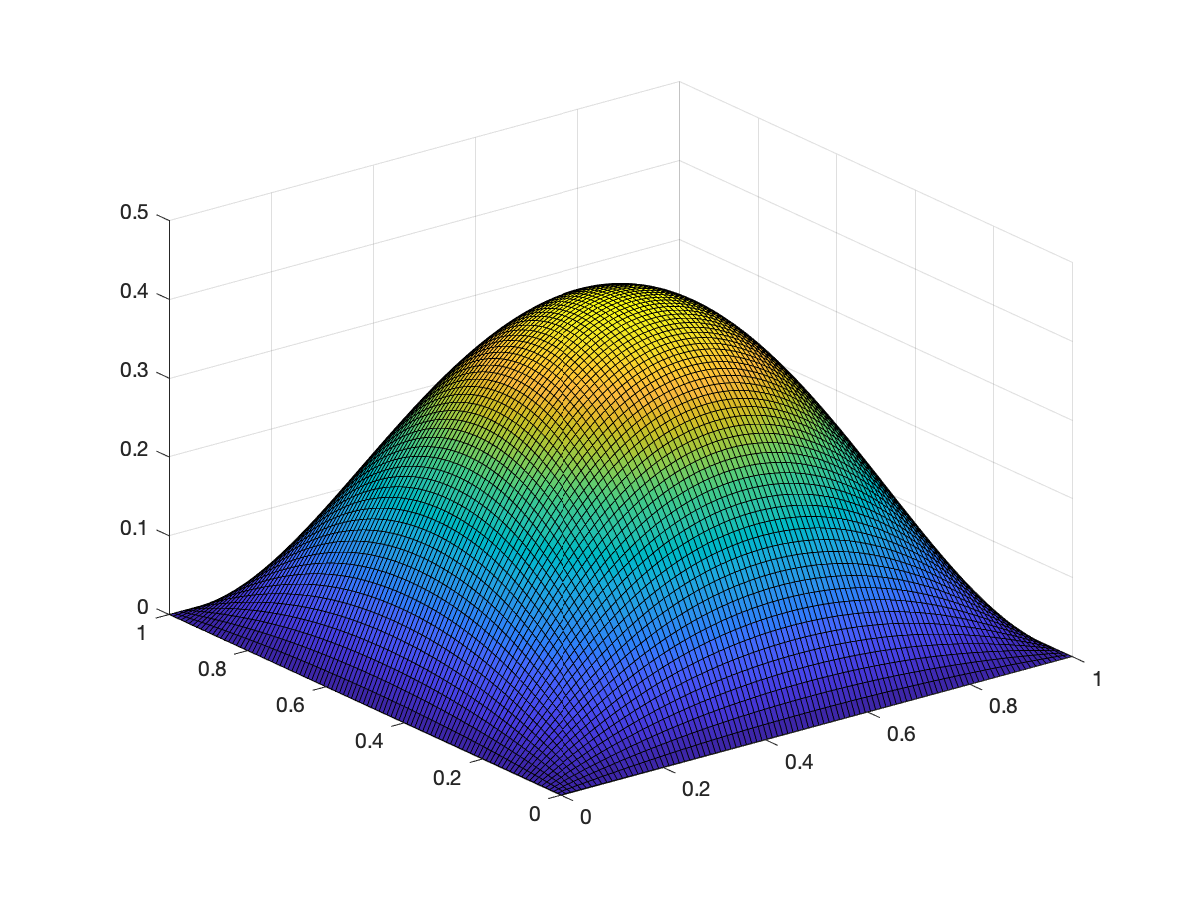
\includegraphics [width=\linewidth] {1608.eps}
      \caption {The Surface Plot at the $1608^{th}$ Iteration Step.}
\end {subfigure}
\caption {The Surface Plots Related to Different Iteration Steps in the Initial Case.}
\label {fig: surface}
\end {figure}
\\From all the discussions and observations above, we could get that with our initial case, the Jacobi method requires lots of steps and a long time to solve the partial differential equation and get the expected optimized images related to the poisson equation. In prder to get a perfect solution with less time, the multogrid algorithm is the best option at least for this initial case at this time.

\subsection {Non-Linear Function}
Now we move to some more complexed problems using the multigrid algorithms, and get a observation about how it could be more powerful in solving the partial differential equations. \\
Similar to the above subsection ``Initial Case", we still set up the functions $u \& f$ at the first time, also we set up the value of the $\epsilon$. Then we compute the partial derivatives $u_{xx}  \  \& u_{yy}$, and get the $u_{xx}+u_{yy}$ assigns to the $\Delta u$. And we keep the boundary conditions the same as we discussed in the previous subsection ``Finite Difference Approximation" inside the section ``Methods".  Then, we set up the $vcycle$ part, we let $r=\Delta u+f$, the following iteration steps are the same as we discussed previously as the ``general steps for the $2-vcycle$". And we consider all of these as the completed code structure for the multigrid algorithm applied in the finite difference approximation. \\
To get a better understanding and impression about this, I listed four surface plots as we continue the iteration steps in the following for observations:
\begin {figure} [h!]
\centering
\begin {subfigure} [b] {0.3\linewidth}
      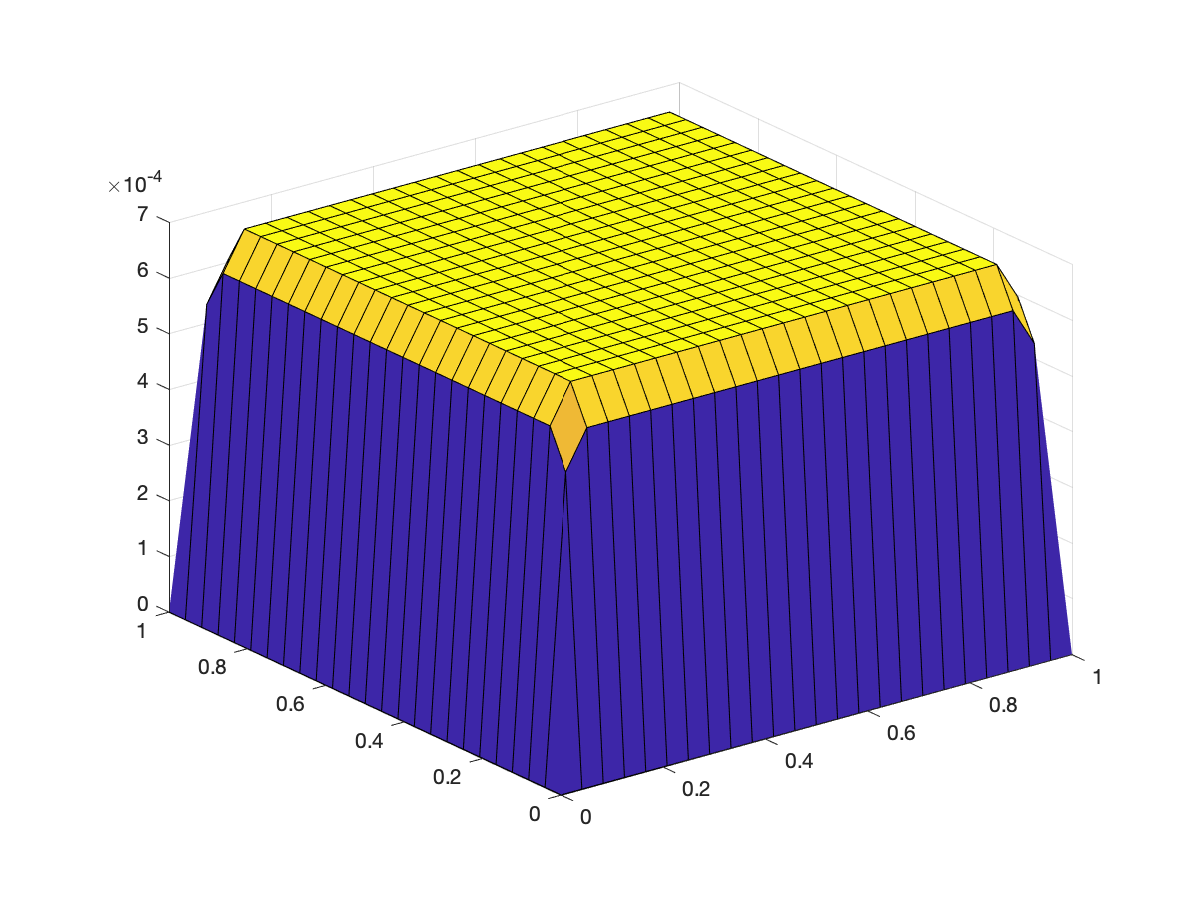
\includegraphics [width=\linewidth] {fda_1.eps}
      \caption {The Surface Plot I.}
\end {subfigure}
\begin {subfigure} [b] {0.3\linewidth}
      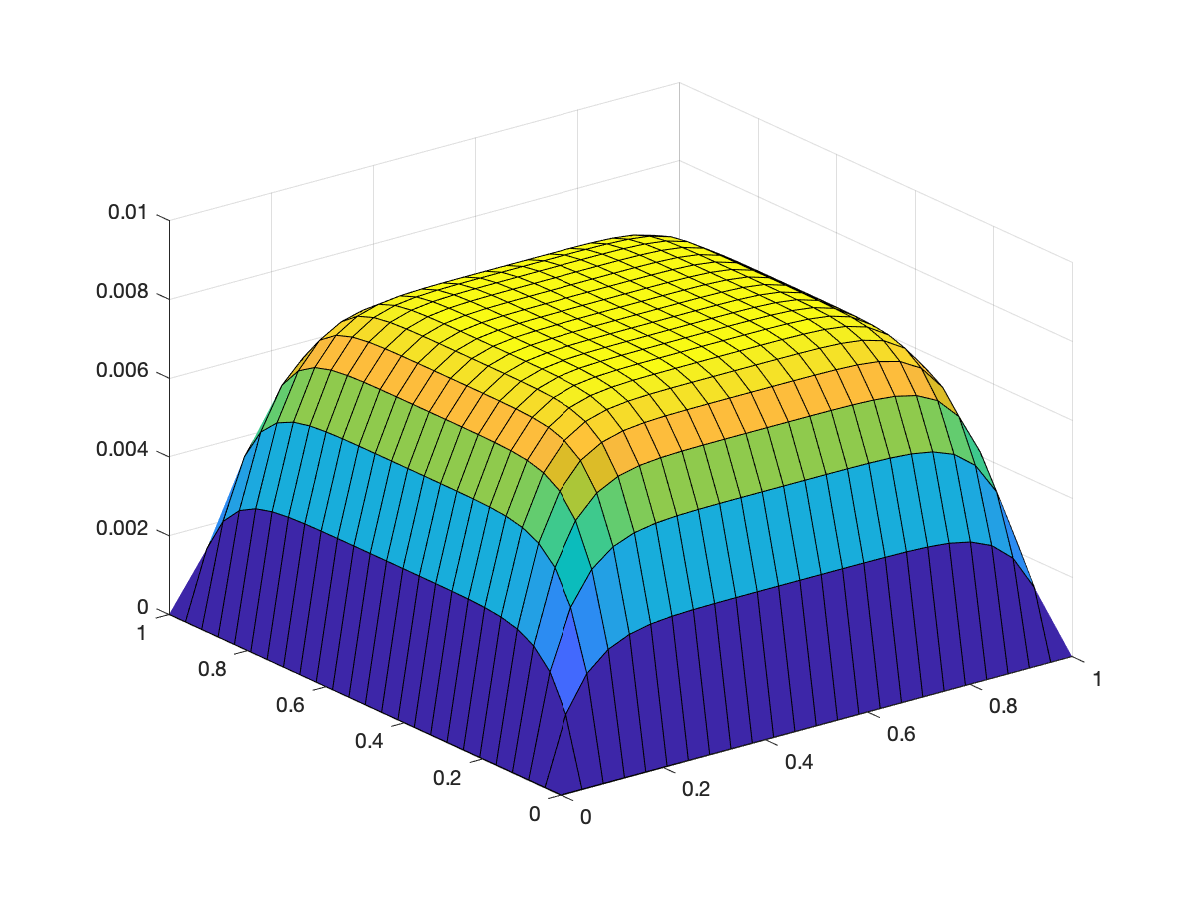
\includegraphics [width=\linewidth] {fda_2.eps}
      \caption {The Surface Plot II.}
\end {subfigure}
\begin {subfigure} [b] {0.3\linewidth}
      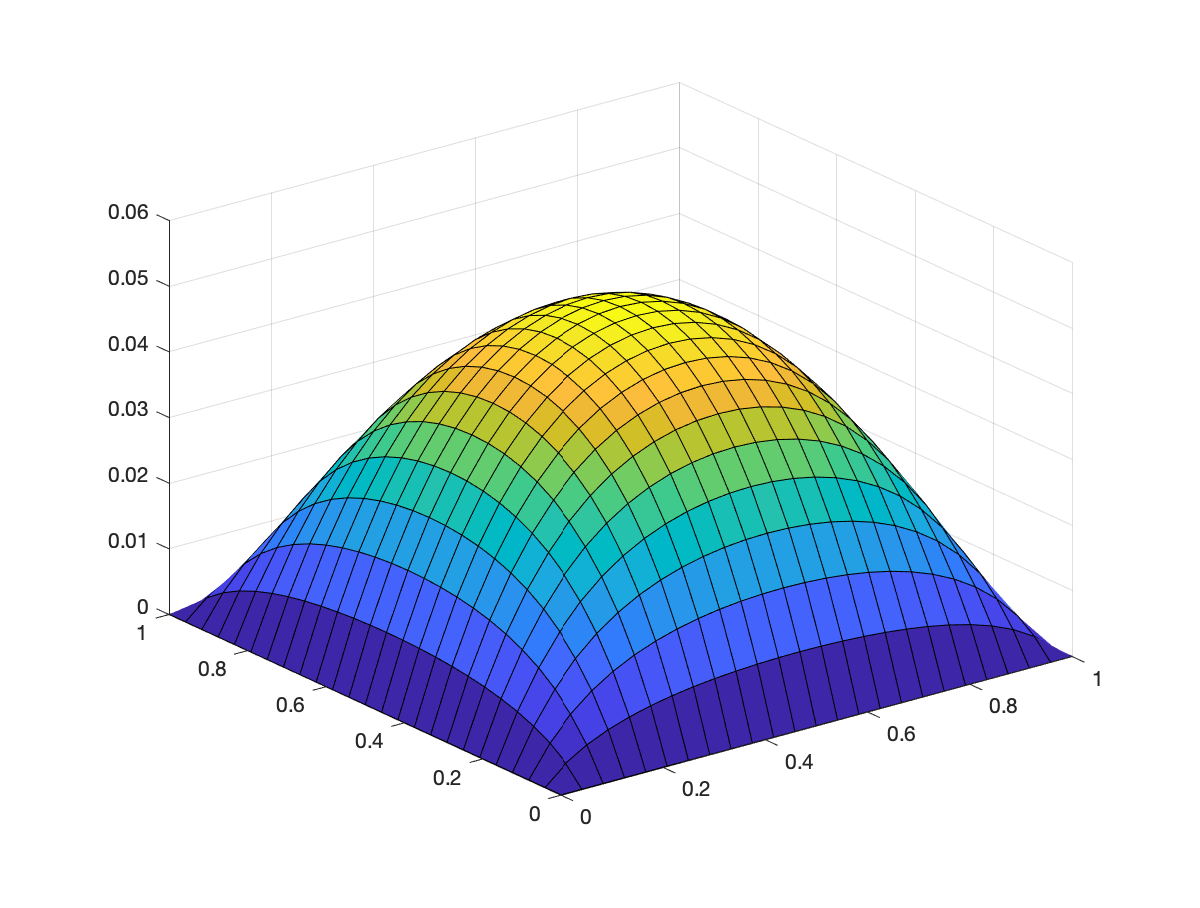
\includegraphics [width=\linewidth] {fda_3.eps}
      \caption {The Surface Plot III.}
\end {subfigure}
\begin {subfigure} [b] {0.3\linewidth}
      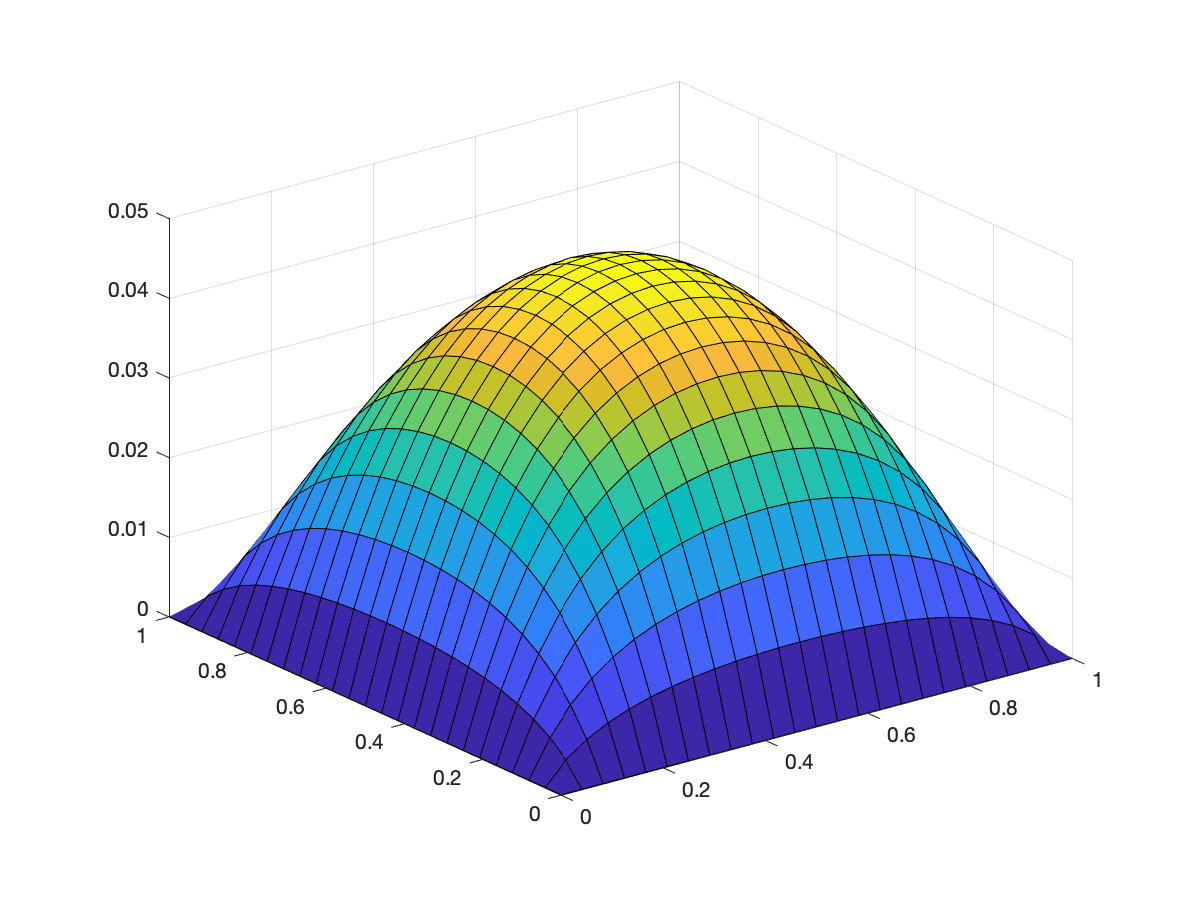
\includegraphics [width=\linewidth] {fda_4.eps}
      \caption {The Surface Plot IV.}
\end {subfigure}
\caption {The Surface Plots Related to Different Iteration Steps in the Finite Difference Approximation.}
\label {fig: surface}
\end {figure}
\\From observing these surface plots above, we could get the impression that with the multigrid algorithm, we could get the expected solution for the poission equation very quickly. To be more scientific and exactly, we could check the exact running time for the multigrid algorithm applied in solving the partial differential equation. And the MatLab returns the exact running time only be $25.995220$ seconds and the elapsed time be much more shorter, which is only the $0.011352$ seconds. \\
Based on these, we could get that the multigrid algorithm is a good option to solve the partial differential equation and optimize the images related to its poisson equation.

\section {Conclusion}
As all above discussions, we could conclude that the multigrid algorithm is an advanced differential equations' solver compared with other iterative methods \footnote {Gauss-Seidel, Jacobi Itetative Methods and the successive overrelaxation (SOR) method} based on variety of data. In any real world imaging processing related to the differential equations, it is obviously that the multigrid algorithm could save the time for the imaging optimization and get the smoothing images much faster than any other methods. 
In general, the multigrid algorithm is mainly focused on solving the non-linear partial differential equations, and could quickly get the expected solution and smoothing images with finite iterations and a limited time, which is a popular algorithm applied in any imagng processing realted to the non-linear partial differential equations' problems.

\begin {thebibliography} {9}

     \bibitem {eM57a}
          Randall~J. LeVeque, \emph {Finite Difference Methods or Ordinary and Partial Differential Equations: \
Steady-State and Time-Dependent Problems}, Philadelphia: Society for Industrial and Applied Mathematics, 2007.

    \bibitem {eM57a}
          Brandt, A., \& Livne, O., \emph {Multigrid Techniques: \
1984 guide with applications to fluid dynamics. Rev. ed., Classics in applied mathematics; 67}, Philadelphia: Society for Industrial and 
Applied Mathematics, 2011.

    \bibitem {sF90}
          Jeffery, Calder, (2018). \emph {Poisson Multigrid Source Code (MATLAB)}, [Source Code], Unpublished.
   
\end {thebibliography}
 
\end {document}